\documentclass{ieee/IEEEtran5/IEEEtran}

\usepackage{amssymb,amsmath,xspace}
%\usepackage{algorithm}
%\usepackage{algorithmic}
%\usepackage{color}
%\usepackage{wrapfig}
\usepackage{subfigure}
%\usepackage{graphicx}
\usepackage{xfrac}
%Tikz 
\usepackage{pgf,tikz}
\usetikzlibrary{shapes,arrows,positioning,backgrounds}

\usepackage[utf8]{inputenc}
\usepackage[hungarian]{babel}
%! own styles
\input{tikz/defs.tik}
%------------------------
\usepackage{paralist}
%\usepackage{soul}
\usepackage[numbers]{natbib}
\usepackage{nccbbb}
%\usepackage{multicol}
%\usepackage{lipsum}

\makeatletter
\renewcommand\bibsection%
{
\section*{\refname
\@mkboth{\MakeUppercase{\refname}}{\MakeUppercase{\refname}}}
}
\makeatother

\definecolor{myTodoColor}{rgb}{1, 0, 0}
\definecolor{linkCol}{rgb}{0.2, 0.0, 0.1}
\definecolor{citeCol}{rgb}{0.3, 0.4, 0.5}
\definecolor{urlCol} {rgb}{0.2, 0.2, 0.5}


%% hyperref package with options!
\usepackage[%
    pdftex,   % which compiler... !dvips!?latex2html?
    raiselinks=true, %
    colorlinks=true, %
    pdftitle={A statisztikus gépi fordítás hatékonyságának jelentés egyértelműsítéssel történő javítása}, %
    pdfauthor={Bordi Eszter and Both Tibor and Pável Szabolcs and Sándor Csanád and Szász Adorján}, %
    pdfkeywords={}, %
    pdfsubject = {technical report}, %
    plainpages=false,%
    pdfpagelabels,%
    citecolor=citeCol,urlcolor=urlCol,linkcolor=linkCol,unicode
]{hyperref} % MUST be the LAST package included



% \newcommand{\vc}[1]{{\ensuremath{\pmb{#1} }}}	
\newcommand{\todo}{\textcolor{myTodoColor}}
\newcommand{\eg}{\textit{e.g.}\xspace}
\newcommand{\ie}{\textit{i.e.}\xspace}
\newcommand{\gp}{\textsc{GP}\xspace}
\newcommand{\nigp}{\textsc{nigp}\xspace}
\newcommand{\mlhgp}{\textsc{mlhgp}\xspace}
\newcommand{\vhgpr}{\textsc{vhgpr}\xspace}
\newcommand{\gpa}{\textsc{GPa}\xspace}
\newcommand{\gph}{\textsc{gp+h}\xspace}
\newcommand{\simex}{\textsc{SimEx}\xspace}
\newcommand{\simexgp}{\textsc{simexGP}\xspace}
\newcommand{\simexgpq}{\textsc{sGP-Q}\xspace}
\newcommand{\simexgpgp}{\textsc{sGP-GP}\xspace}
\newcommand{\matlab}{\textsc{matlab}\xspace}
\def\tr{\ensuremath{\mathop{\mathrm{tr}}}}


%opening
\title{A statisztikus gépi fordítás hatékonyságának jelentés egyértelműsítéssel történő javítása}
\author{Bordi Eszter, \and Both Tibor, \and Pável Szabolcs, \and Sándor Csanád és \and Szász Adorján \\ Matematika és Informatika Kar, Babe\c{s}-Bolyai Tudományegyetem, Kogalniceanu 1, 400084 Cluj-Napoca, Romania \\ \textsc{bordieszter@gmail.com}, \textsc{bothtibi@yahoo.com}, \textsc{\{pszabolcs93,scsanad\}@gmail.com}, \textsc{szasz\_adorjan@yahoo.com}}
%\thanks{a}
% \institute{Faculty of Mathematics and Informatics, Babe\c{s}-Bolyai University, Kogalniceanu 1, 400084 Cluj-Napoca, Romania \\
% \email{\{bboti,jakabh,csatol\}@cs.ubbcluj.ro}}

\newcommand{\vc}[1]{{\ensuremath{\pmb { #1 } }}}

\begin{document}

\maketitle

\begin{abstract}
A statisztikus gépi fordítás (SMT) olyan gépi fordítás, amely statisztikai modellekre alapul. A módszer hatékonyságának növelése érdekében beépítettük alkalmazásunkba a wikipedia alapú szóegyértelműsítést (WSD).
  
\end{abstract}

%%%%%%%%%%%%%%%%%%%%%%%%%%%%%%%%%%%%%%%%%%%%%%%%%%%%%%%%%%%%%%%%%%%%%%%%%%%%%%%%%%%%%%%%%%%%%%%%%%%%%%%%%%%%%%%%%
%%%%%%%%%%%%%%%%%%%%%%%%%%%%%%%%%%%%%%%%%%%%%%%%%%%%%%%%%%%%%%%%%%%%%%%%%%%%%%%%%%%%%%%%%%%%%%%%%%%%%%%%%%%%%%%%%
\section{Bevezetés}
Gépi fordítást elsősorban szövegek megértésének elősegítésére, információszerzésre használják, jelenleg nem alkalmas emberi fordítással azonos minőségű fordítás létrehozására. A statisztikus gepi forditas ennek egyik ága, amely a fordítást statisztikai modellek segítségevel végzi.
A legfőbb nehézséget a többértelmű szavak, valmint a kifejezések fordítása okozza.
A legnagyobb fejlődést  statisztikus gepi forditas számára az jelentette, amikor a modelleket szavak helyett a szókapcsolatokra kezdték építeni. Azonban ezek a modellek még mindig nem veszik figyelmebe a szavak/kifejezések többértelműségét, ezért hozzáadtuk a szövegegyértelműsítés módszerét is. A wikipedia adathalmaza lett felhasználva, mivel az egyik legnagyobb létező adathalmaz, amely elérhető több nyelven is. 

Ebben a cikkben elemezzük eredményeinket, melyből látható, hogy a szövegegyértelműsítés használatával növelhető a statisztikus gépi fordítás hatékonysága.

%%%%%%%%%%%%%%%%%%%%%%%%%%%%%%%%%%%%%%%%%%%%%%%%%%%%%%%%%%%%%%%%%%%%%%%%%%%%%%%%%%%%%%%%%%%%%%%%%%%%%%%%%%%%%%%%%
%%%%%%%%%%%%%%%%%%%%%%%%%%%%%%%%%%%%%%%%%%%%%%%%%%%%%%%%%%%%%%%%%%%%%%%%%%%%%%%%%%%%%%%%%%%%%%%%%%%%%%%%%%%%%%%%%
\section{A modell definiálása és letező megoldások} \label{sec:model_definition}

\subsection{A statisztikus gépi fordítás}

A statisztikus módszerek használatát a gépi fordításban legelőször Warren Weaver, egy levélben javasolta az 1949-es években. Azonban az elméleti nehézségeknek és az akkori számítógépek fejlettségének tulajdoníthatóan a módszert csak 1990-ben próbálták ki.

Az általunk felhasznált modell -- a kifejezés alapú fordító modell -- a zajos csatorna modellen alapszik -- \ref{fig:modell:fig1}. Tételezzük fel, hogy egy $F$ nyelv valamilyen $f$ szövegének fordítása egy $E$ célnyelvbe az $e$-vel jelölt szöveg. Annak valószínűsége, hogy $f$-et lefórdítva $e$-t kapunk: $P(e|f)$. Felhasználva Bayes képletét a feltételes valószínűség a következő alakban írható:

\begin{equation}
	P(e|f) = \frac{P(e)P(f|e)}{P(f)}
\end{equation}

Az nevezőt elhagyva a következő optimalizálási feladathoz jutunk:

\begin{equation}
	T(f) = argmax_e P(e|f) = argmax_e P(e)P(f|e)
\end{equation} 

Ezzel a feladatunkat három részre osztható: 
\begin{itemize}
	\item
		Nyelvi modell: $P(e)$
	\item
		Fordítási modell: $P(f|e)$
	\item
		Dekóder: $argmax$
\end{itemize}














\begin{figure}[b]
  	\centering
  		\pgfimage[width=0.6\linewidth]{images/smt_translation_model}
  	\caption[smt_translation_model]%
  	{A zajos csatorna modell}
 	\label{fig:modell:fig1}
\end{figure}





\subsection{Jelentés egyértelműsítés}
bemutatni a wsd-t?

\subsection{Létező megoldások}
jelenlegi phrase based megoldasok
	miert jok, miert nem
	osszehasonlitasok mas modszerekkel
milyen probalkozasok vannak a wsd beepitesere?
mennyire jok ezek?


%%%%%%%%%%%%%%%%%%%%%%%%%%%%%%%%%%%%%%%%%%%%%%%%%%%%%%%%%%%%%%%%%%%%%%%%%%%%%%%%%%%%%%%%%%%%%%%%%%%%%%%%%%%%%%%%%
%%%%%%%%%%%%%%%%%%%%%%%%%%%%%%%%%%%%%%%%%%%%%%%%%%%%%%%%%%%%%%%%%%%%%%%%%%%%%%%%%%%%%%%%%%%%%%%%%%%%%%%%%%%%%%%%%
\section{Saját módszer} \label{sec:new_method}

Ebben a részben részletezzünk az általunk implementált módszert. A cél egy olyan rendszer felépítése, amely a már meglévő statisztikus gépi fordítás rendszereket egészíti ki egy jelentés-egyértelműsítést szolgáltató (WSD) rendszerrel. Az SMT rendszerek gyakran rossz eredményt adnak abban az esetben, amennyiben a fordítandó szavak több jelentéssel is bírnak. Ezekben az esetekben nyújthat segítséget egy ilyen bővítmény, amely képes a szövegkörnyezet alapján meghatározni a szó tényleges jelentését, és így egy pontos fordítást adni az adott mondatra. 

Tárgyaljuk a felhasznált Wikipedia alapú WSD modult, valamint részletezzük annak alkalmazását egy meglévő SMT rendszerben.

\subsection{Wikipedia alapú jelentés-egyértelműsítés} \label{sec:WikiWSD}

Egy korábbi munkában \cite{Gabrilovich:2007:CSR} bevezettek egy Wikipedia oldalakon alapuló módszert, amelyben a cikkek címeit mint fogalmakat tekintették, amelyeket egy adott szó jelentésének leírására használták fel. A Wikipedia esetünkben is egy jó megoldásnak bizonyult, hiszen a világ egyik legnagyobb nyílt enciklopédiája (az angol változat több, mint 400 millió szót és több, mint 1 millió cikket tartalmaz), a tartalom különböző cikkekbe van rendezve, és ami a számunkra legfontosabb, hogy ugyanazok a cikkek több nyelven is elérhetőek, és ezek között a cikkek között egy jól meghatározott megfeleltetés is van. Ezekből az okokból kifolyólag mi is egy hasonló rendszer alkalmazása mellett döntöttünk.

A cél egy szemantikus értelmező építése, amely képes egy szóhoz vagy egy szövegrészlethez egy súlyozott fogalomvektort hozzárendelni. A vektor elemei az adott szövegrészlethez kapcsolódó fogalmak lesznek, míg a súlyok azt határozzák meg, hogy mennyire jellemző az adott fogalom a szövegre. Amikor fogalmakról beszélünk továbbra is a cikkek címét értjük. 

Minden Wikipedia cikket egy attribútum vektorként reprezentálhatunk. A vektor minden eleme megadja, hogy az elemhez tartozó szó mennyire releváns a cikk címe által reprezentált fogalomra. A relevanciát a szóhoz tartozó TFIDF súllyal fejezzük ki. Jelölje $k_t$ az $t$ szóhoz tartozó TFIDF súlyt. Ekkor 
\begin{equation}
	k_t = \frac{tf_t}{df_t}
\end{equation}
ahol $tf_t$ a $t$ szó előfordulásainak a száma a cikkben, míg $df_t$ azoknak a dokumentumoknak a száma, amelyben $t$ előfordul.

Ahhoz, hogy a szemantikus értelmezést gyorsabban el tudjuk végezni, egy invertált indexet építünk fel, vagyis minden szóhoz egy fogalomlistát rendelünk, amelynek mindegyik eleme az adott fogalom és a szó TFIDF súlya az adott fogalomhoz tartozó cikk esetében. Ezen kivül, hogy a felhasznált tárhelyet megfelelően alacsonyan tudjuk tartani, csak azokat a fogalmakat őrizzük meg ebben a listában, ahol a hozzárendelt súly átlép egy küszöbértéket (\ref{fig:invindex}. ábra).

\begin{figure}[ht]
	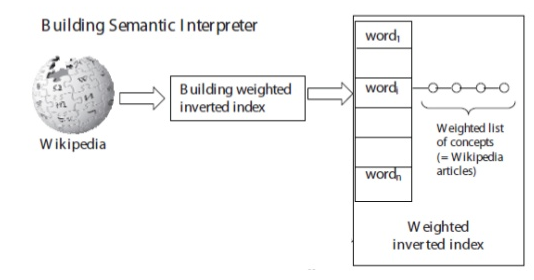
\includegraphics[scale=0.3]{images/invindex} 
	\caption{Invertált index}
	\label{fig:invindex}
\end{figure}		

Mivel a fordítás során a bemeneti szövegek nyelve különböző, fel kell építenünk egy invertált indexet minden nyelvhez, amit használni szeretnénk. Ehhez fontos az is, hogy legyen egy megfeleltetésünk a különböző nyelvű cikkek és ezáltal fogalmak között, ezt azonban a Wikipedia felépítése direkt módon megadja.

Két szöveg összehasonlításához szükséges, hogy az egyes szövegekhez hozzá tudjunk rendelni egy fogalomvektort. Jelölje $T = \{w_i\}$ a bemeneti szöveget, ahol $w_i$ egy szó. Minden $w_i$ szóhoz társítsuk a $v_i$ TFIDF súlyt, ahol a $tf_i$ tagot ezúttal a szó előfordulásainak számát jelenti a bemeneti szövegben. Minden szóhoz társítsunk egy $k_{i,j}$ elemekből álló vektort, ahol egy elem az $w_i$ szó $c_j$ fogalmomhoz tartozó súlyát jelenti az invertált index alapján. A teljes szöveg súlyvektorának $j.$ komponensét ekkor a 
\begin{equation}
\sum_{w_i \in T} v_i \cdot k_{i,j}
\end{equation}
adja (\ref{fig:textfragment}. ábra)

\begin{figure}[ht]
	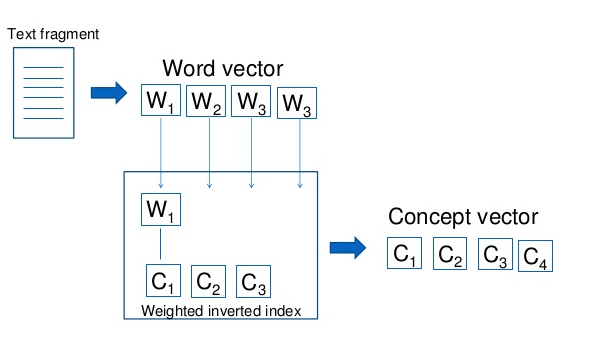
\includegraphics[scale=0.3]{images/textfragment}
	\caption{Fogalomvektor felépítése bemeneti szöveg alapján}
	\label{fig:textfragment}
\end{figure}	

Az előbb leírt módon előállított súlyvektorokat felhasználva a két vektor koszinusz távolságának kiszámolásával megadhatjuk a két szöveg szemantikai hasonlóságát (\ref{fig:similarity}. ábra). Legyen $\overrightarrow{u}$ és $\overrightarrow{v}$ a két súlyvektor, ekkor a két szöveg hasonlósága: 
\begin{equation}
	sim_{u,v} = \frac{\overrightarrow{u} \cdot \overrightarrow{v}}{\left\lVert \overrightarrow{u} \right\rVert \cdot \left\lVert \overrightarrow{v} \right\rVert}
\end{equation}

\begin{figure}[ht]
	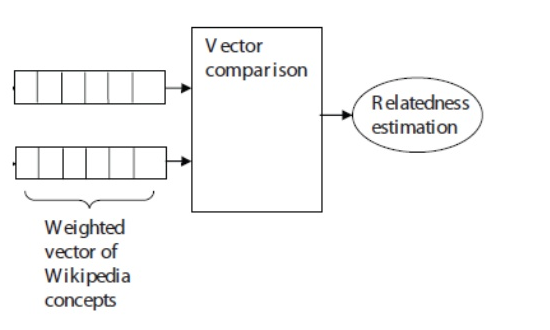
\includegraphics[scale=0.3]{images/similarity}
	\caption{Hasonlóság meghatározása súlyvektorokból}
	\label{fig:similarity}
\end{figure}	

\subsection{WSD modul beépítése SMT rendszerbe} \label{sec:WSDinSMT}

Az egyik legegyszerűbb és jól működő modell a jelentés-egyértelműsítés SMT-rendszerekbe való integrációjára az $n$ legjobb elem újrarangsorolása (\cite{apidianaki2012wsd}).

Első lépésként felhasználjuk a standard SMT-rendszerünket, amely segítségével kapunk $n$ darab lehetséges fordítást a bemeneti szövegre. Az így kapott fordításokat és a bemeneti szöveget felhasználva a \ref{sec:WikiWSD}. részben tárgyalt módszer segítségével minden fordításhoz hozzárendelhetünk egy súlyt. Az SMT által és a WSD által adott súlyokat is normalizáljuk, majd ezeket összeadjuk. A végső fordítás az így kapott súlyok szerinti legjobb eredmény lesz:

\begin{equation}
	f = argmax_i (\frac{w_{SMT, i}}{\left\lVert w_{SMT} \right\rVert} + \frac{w_{WSD, i}}{\left\lVert w_{WSD} \right(\rVert})
\end{equation}



%%%%%%%%%%%%%%%%%%%%%%%%%%%%%%%%%%%%%%%%%%%%%%%%%%%%%%%%%%%%%%%%%%%%%%%%%%%%%%%%%%%%%%%%%%%%%%%%%%%%%%%%%%%%%%%%%
%%%%%%%%%%%%%%%%%%%%%%%%%%%%%%%%%%%%%%%%%%%%%%%%%%%%%%%%%%%%%%%%%%%%%%%%%%%%%%%%%%%%%%%%%%%%%%%%%%%%%%%%%%%%%%%%%
\section{Eredmények} \label{sec:results}

%%%%%%%%%%%%%%%%%%%%%%%%%%%%%%%%%%%%%%%%%%%%%%%%%%%%%%%%%%%%%%%%%%%%%%%%%%%%%%%%%%%%%%%%%%%%%%%%%%%%%%%%%%%%%%%%%
%%%%%%%%%%%%%%%%%%%%%%%%%%%%%%%%%%%%%%%%%%%%%%%%%%%%%%%%%%%%%%%%%%%%%%%%%%%%%%%%%%%%%%%%%%%%%%%%%%%%%%%%%%%%%%%%%
\section{Következtetések} \label{sec:conslusions}

%%%%%%%%%%%%%%%%%%%%%%%%%%%%%%%%%%%%%%%%%%%%%%%%%%%%%%%%%%%%%%%%
%%%%%%%%%%%%%%%%%%%%%%%%%%%%%%%%%%%%%%%%%%%%%%%%%%%%%%%%%%%%%%%%
\bibliographystyle{splncsnat}
% \bibliographystyle{IEEEtran}

\bibliography{main}

\end{document}